\documentclass{article}
\usepackage{graphicx}
\usepackage[utf8]{inputenc}
\usepackage[T1]{fontenc}
\usepackage[francais]{babel}
\usepackage{layout}
\usepackage{caption}
\usepackage{subcaption}

\begin{document}
\begin{titlepage}
\begin{center}
\Huge Rapport TPA phase 1

\normalsize
\vspace{0.5cm}
\Large {\underline{ Groupe 3 Bleu : Sokoban} }

\vspace{1cm}

\normalsize
Goron Nathan, De La Rosa Louis-David, Basset Emilien, Demé Quentin

\vspace{1cm}
\begin{center}
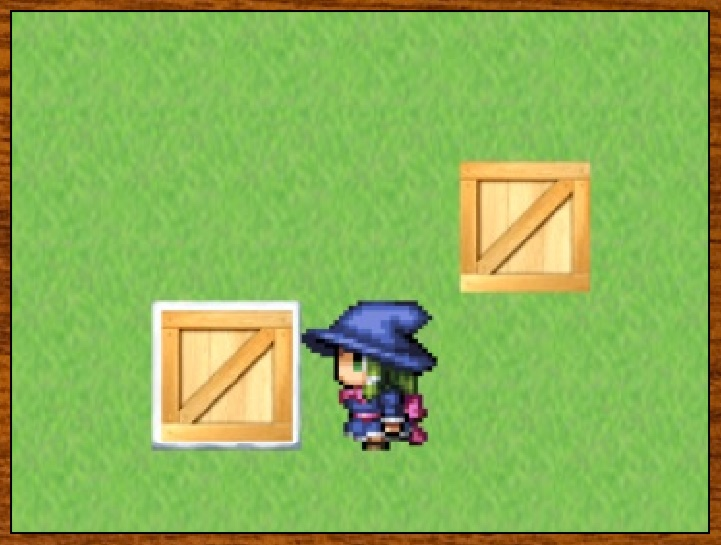
\includegraphics[scale=0.7]{../Screenshots/main.jpg}
\end{center}
\vspace{3.5cm}
L2 informatique 2016-2017 Université de Caen Basse-Normandie
\end{center}
\end{titlepage}


\newpage
\tableofcontents

\newpage
\begin{center}
	\section{Introduction}
\end{center}
\vspace{1cm}
	Parmi les projets proposés, nous avons fait le choix d'éviter les projets n'étant pas des jeux de peur qu'ils limitent notre créativité et notre motivation quant a son développement. Le jeu de Sokoban nous paraissait être un projet ambitieux et intéressant de par la difficulté dans l'implémentation de son IA.
 \vspace{0.5cm}

	Il s'agissait donc de développer un Jeu de Sokoban: Un jeu de puzzle dans lequel un personnage déplace un certains nombres de caisses sur des emplacements dans un niveau fermé, le joueur gagne la partie si il parvient à boucher tous les emplacements avec les caisses.
	
	Après avoir songé à l'utilisation du moteur de jeu Unreal Engine, nous avons décidé de développer ce projet en Python avec l'aide de la librairie PyGame qui offre une grande liberté dans l'interface graphique ainsi que de nombreuses méthodes facilitant les mécaniques de fonctionnement de base d'un jeu. 
	\newpage
	\begin{center}
	\section{Cahier de charges}
	\end{center}
	\vspace{1cm}
		\subsection{Déroulé fonctionnel, objectif}
		Le programme sera écrit en Python à l’aide de la librairie Pygame et répondra aux critères suivants d’ici la version finale de son développement:
			\subsubsection{Phase 1:}
			Le jeu sera jouable par humain via un prototype non-définitif(changements possibles en phase2), le joueur pourra se déplacer dans un niveau importé au format .slc composé de plusieurs éléments (expliqués dans les détails de fonctionnement du moteur de jeu).
			\subsubsection{Phase 2:}
			Le jeu se verra ajouter une fonctionnalité de résolution automatique grâce à l’algorithme A* et aux heuristiques, cet algorithme proposera un chemin qui soit parmis les meilleurs, et ce le plus rapidement possible (dans la plupart des cas en fonction de la difficulté)pour compléter le niveau. Cet algorithme devra être anytime , c'est-à-dire capable de compléter un niveau quelque soit son point de départ.
Les fonctionnalités additionnelles facultatives sont listées dans la catégorie
"Fonctionnalités additionnelles".
		\subsection{Contexte de réalisation}
		Ce projet est réalisé dans le cadre de l’évaluation de la valeur "TPA" en L2 info 2016-2017 de l’université de Caen.
		\subsection{Découpage}
		Le programme sera composé des modules suivants : \newline
— Le module sokoban qui assurera le fonctionnement général du programme
(moteur de jeu, conditions de victoire,interface graphique, importations
des niveaux). \newline
— Le module classes qui comprendra toutes les classes et méthodes nécessaire
au fonctionnement du jeu. \newline
— Le module constantes stockant les importations d’images pour les personnages
et les cases ainsi que les variables nécessaire pour les variations
de tailles de niveaux a l’écran. \newline
-Le module Sokobastar qui gérera le 
Ce découpage pourra être modifié en fonction des choix de fonctionnalités additionnelles. \newline
		\subsection{Pré-requis d'utilisation}
		Le jeu fonctionnera sous n’importe quel système muni de python(2.7 a 3.5) et de la librairie Pygame. Le jeu sera intuitif d’utilisation et ne nécessitera aucune connaissance informatique particulière.
		\subsection{Règles du jeu}
		Le joueur déplace un personnage dans un niveau constitué de murs, de cases
vides, de caisses et de socle pour les caisses. Il faudra déplacer les caisses dans
le niveau afin de couvrir tous les socles pour terminer le niveau. Le joueur ne peut que pousser et non tirer. De plus, il ne peut pousser qu’une seule caisse à la fois. Ces règles impliques que le joueur peut se trouver bloquer.
		\subsection{Fonctionnalités additionnelles}
			6 Fonctionnalité additionnelles: \newline
Les fonctionnalités suivantes seront susceptible d’être implémentée d’ici la
version finale du programme: \newline
— Menu permettant le choix du niveau et la modifications d’éventuelles
options(sons , design de la fenêtre...). \newline
— Bouton "undo" permettant d’annuler le dernier mouvement du joueur. \newline
— Système de sauvegarde pour conserver son avancée dans un niveau. \newline

		\subsection{Calendrier , dates fixées:}
		Le développement du jeu est découpé en deux phases: \newline
- Phase 1/1er semestre: réalisation d’un jeu jouable par un humain et recherches
sur l’IA (A* , heuristiques), importation des niveaux. \newline
-phase 2/2nd semestre: programmation de la résolution automatique anytime et ajout d'éventuelles fonctionnalités additionnelles.\newline
		\subsection{Internationalité}
		Internationalité :
Le jeu ne sera pas traduit et sera utilisable uniquement en Français.
		\subsection{Priorités, importances relatives des fonctionnalités}
		Le fonctionnement du jeu sans IA et la possibilité d’importation des niveaux sont prioritaires, la résolution automatique ne sera programmée qu’ensuite. Les fonctionnalités additionnelles ne seront développées qu’une fois les objectifs des deux phases remplies.
	\newpage
	\begin{center}
	\section{Détails du fonctionnement}
		\vspace{0.5cm}
		Pour des raisons de clarté et de facilitation d'implémentation , nous avons choisi d'implémenter notre programme en orienté objet plutôt qu'en procédural.
		\end{center}
		\vspace{0.5cm}
		\subsection{Découpage et fonctionnement du moteur de jeu}
		
			Notre moteur de jeu repose sur 5 classes:
			\begin{itemize}
				\item Sprite 
				\item Personnage 
				\item Caisse
				\item Niveau
				\item LevelCollection
				\end{itemize}
				\vspace{0.5cm}
			Les classes Sprite, Personnage et Caisse servent a représenter visuellement les objets suivants:
				\begin{itemize}
					\item Le personnage - Il représente le personnage contrôlé par le joueur
					\item Les caisses - Les entités manipulable par le personnage
					\item Les murs - Moteur de difficulté du jeu ; Ils bloquent le déplacement des caisses et du personnage
					\item Les cibles - Emplacements sur lesquels il faut placer les caisses
					\item Les cases vides - Cases sur lesquels les personnage et caisses peuvent se déplacer
				\end{itemize}
				\vspace{0.5cm}
				La continuité du jeu est controlée par la variable continuer, celle-ci est établie a 1 au lancement du jeu et a 0 lorsque le joueur compléte le niveau : a ce moment , le jeu se ferme et affiche un message de victoire en console
				
				Pour construire notre plan de jeu , nous avons choisi de décomposer notre niveau en 2 grilles nommées GameP et GameO contenant a elles deux les objets cités plus haut ; la grille gameP(game plan)contient les cibles et les espaces vides tandis que la grille gameO(game Obstacle) contient les murs, les caisses et le personnage .L'affichage du niveau consiste donc en la superposition des deux plans et permet ainsi une vérification de victoire plus facile a la fin du jeu : 
				\begin{figure}
				
				\begin{center}
					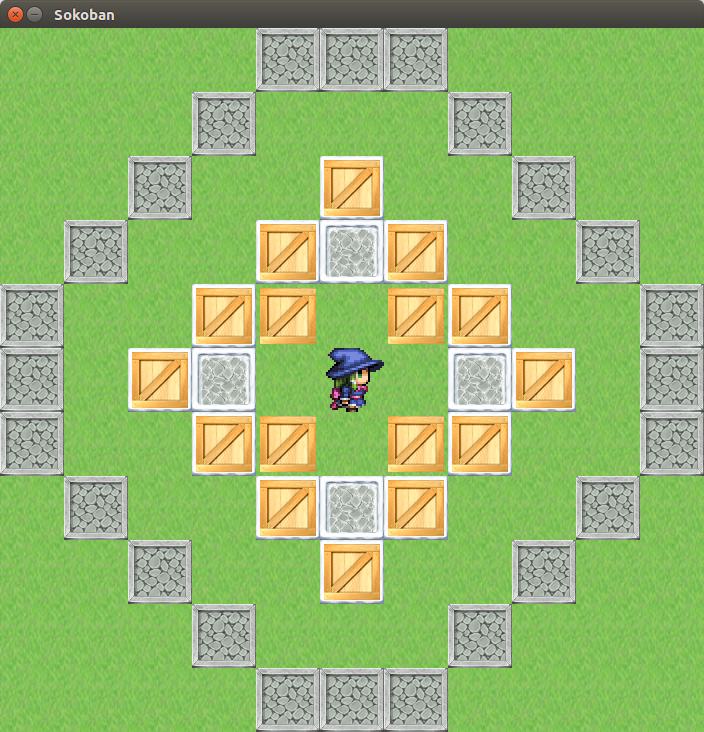
\includegraphics[scale=0.25]{../Screenshots/05.png}
						\caption{Apercu des deux grille superposées}
					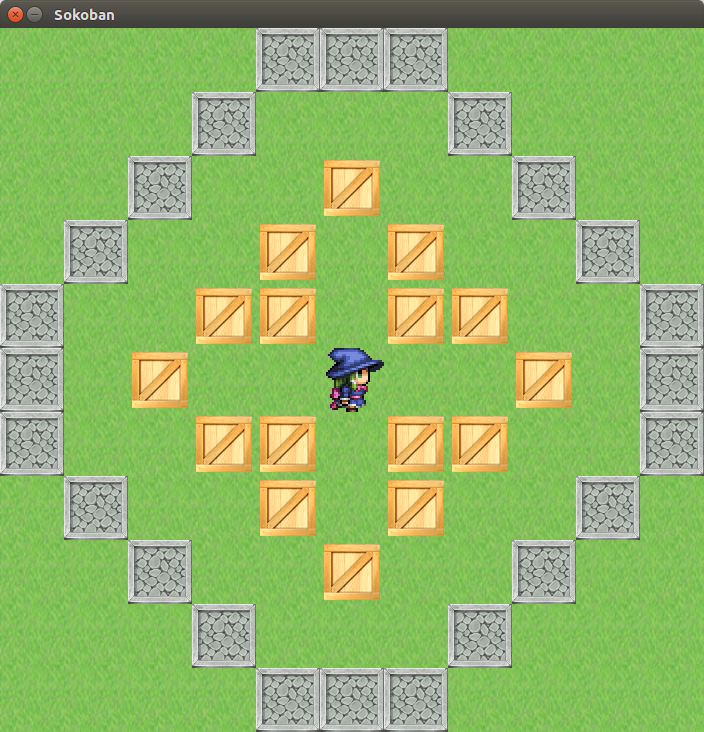
\includegraphics[scale=0.25]{../Screenshots/06.png}
						\caption{Apercu de la grille GameO}
					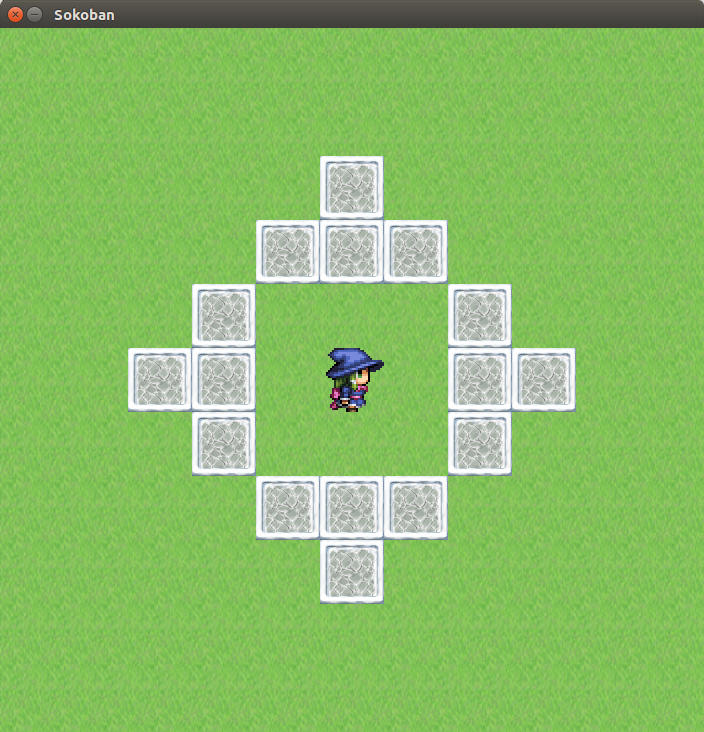
\includegraphics[scale=0.25]{../Screenshots/07.png}
						\caption{Apercu de la grille GameP}
				\end{center}
				\end{figure}
				\newpage
		\subsection{Communication joueur-jeu , utilisation du programme}
		
			Pour les déplacements du personnage nous utilisons la méthode event.key de PyGame qui permet de gérer des événements liées a l'utilisation du touches du clavier , 6 touches événement sont actuellement gérés : touche directionnelle droite(K-RIGHT : déplacement du personnage vers la droite) ,touche directionnelle gauche(K-LEFT : déplacement du personnage vers la gauche) ,touche directionnelle haut(K-UP : déplacement du personnage vers le haut) ,touche directionnelle bas(K-DOWN: déplacement du personnage vers le bas) ,   pavé numérique(KP-MULTIPLY: lance la résolution automatique du niveau avec Astar) et la touche échap(KP-ESCAPE : fermeture du jeu)
		\subsection{fonction et restriction de déplacement du personnage}		
		Lorsque le joueur presse une des touche événement de déplacement citées plus ci-dessus , la méthode spéciale déplace() de la classe Personnage retournant un booléen est appelée pour vérifier si le déplacement est autorisé de la maniére suivante:
	\vspace{0.5cm}
	\begin{center}

			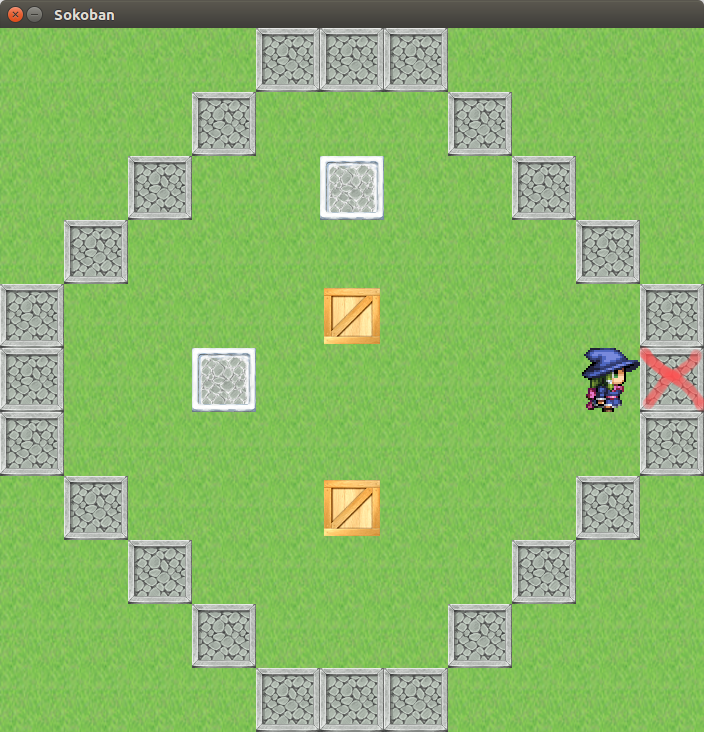
\includegraphics[scale=0.25]{../Screenshots/01.png}
				
	\end{center}
		\subsection{mécanique de déplacement des caisses}
			Le déplacement des caisses est régie selon les règles suivantes : 
			\begin{itemize}
				
				\item Le joueur ne peux pas tirer les caisses, Le joueur perd donc la partie si il pousse une caisse sur une case de coin qui n'est pas une stelle
				\item Le joueur ne peux pousser qu'une seule caisse a la fois 
				
				\end{itemize}
				
				
				
				
	\begin{figure}		
	
Dans le même ordre idée que pour la classe Personnage , la classe Caisse est dotée d'une méthode spéciale déplace() vérifiant si le déplacment d'une caisse est autorisé:
 A partir de la position du joueur et de la direction du déplacement demandé , la fonction vérifie d'abord si la prochaine case est bien une caisse et ensuite si la case suivante est une case vide ou une case stelle , si cette condition est vérifié le déplacement de la caisse s'effectue comme exposé ci dessous:

	\begin{center}
	\begin{minipage}[b]{0.4\textwidth}
    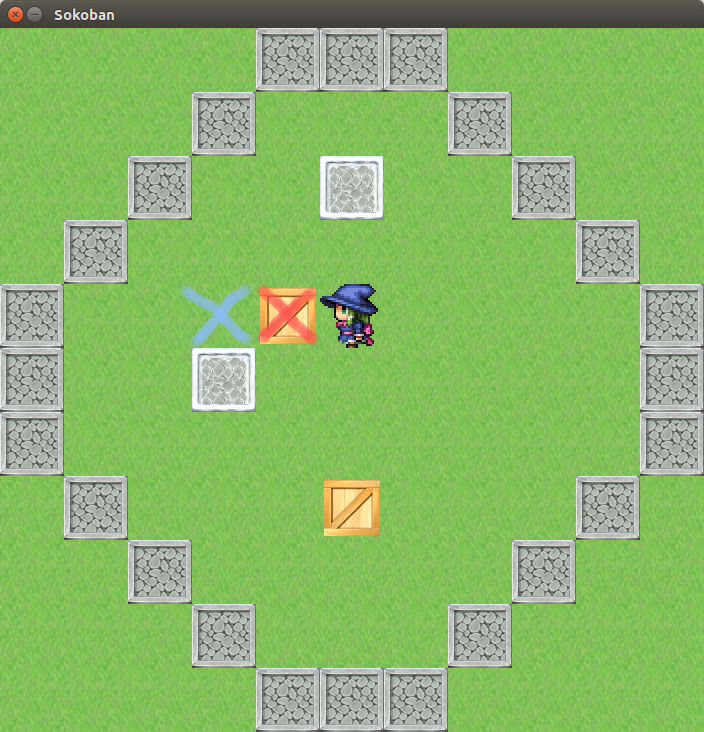
\includegraphics[width=\textwidth]{../Screenshots/02.png}
    \caption{déplacement autorisé}
  \end{minipage}
  \hfill
  \begin{minipage}[b]{0.4\textwidth}
    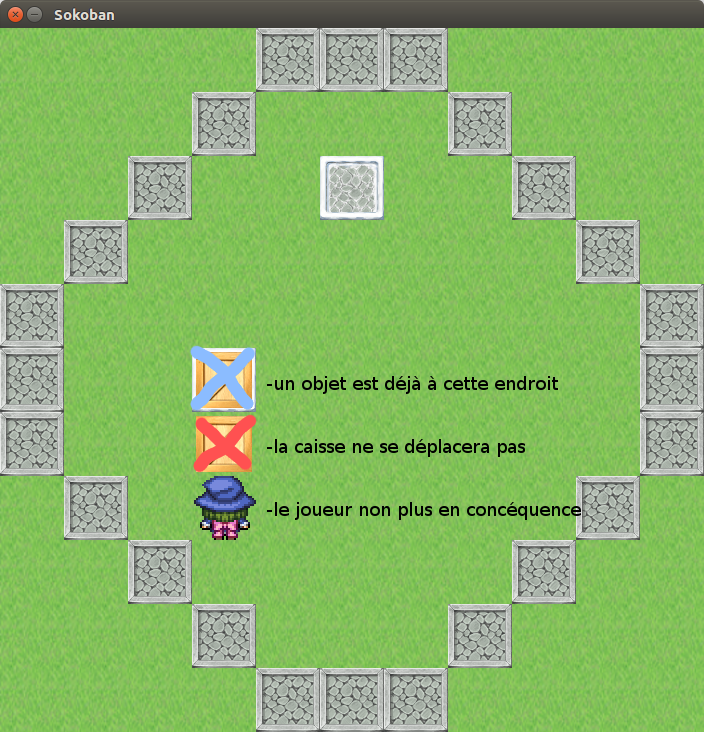
\includegraphics[width=\textwidth]{../Screenshots/04.png}
    \caption{déplacement impossible}
  \end{minipage}
				
				
							
	\end{center}
	\end{figure}	
		
		
		
		
			
	\newpage
		\subsection{Astar}
		
		\newpage
	\section{Schéma UML}
	\newpage
	\begin{center}
	\section{Perspectives d'améliorations en phase 2}
	\end{center}
	\vspace{1cm}
	 Aprés l'implémentation des heuristiques d'Astar , nous pourrons travailler sur les éventuelles possibilités d'améliorations évoquées dans le cahier des charges :
	 \vspace{0.5cm}
	 \begin{itemize}
	 	\item\underline{Ajout d'un menu principal:} Un menu s'affichant au lancement du jeu répertoriant plusieurs catégories ; le menu de jeu dans lequel on choisira le niveau dans lequel on souhaite jouer , un menu d'option pour régler des paramètres d'affichage ou changer le sprite de son personnage et un menu statistiques dans lequel le joueur pourra consulter ses haut-faits ou ses meilleurs scores sur les niveaux
	 	\vspace{0.5cm}
	 	\item\underline{Sons et musique:}Agrémenter le jeu d'une bande son ainsi que d'effets sonores correspondant au actions du personnage paramétrable  dans les options 
	 	\vspace{0.5cm}
	 	\item\underline{Fonctionnalité "undo":}Possibilité pour le joueur d'annuler son dernier coup si jamais il se retrouve bloqué ou souhaite optimiser son parcours
	 	\vspace{0.5cm}
	 	\item\underline{Interface HUD:}Interface en jeu donnant au joueur un certain nombre d'informations relatives a ses performances : temps de jeu depuis le lancement du niveau , nombre de coup joué , nombre de stelles restantes activer ...
	 	\vspace{0.5cm}
	 	\item\underline{Sauvegarde de l'avancement:}Pour les niveaux difficiles , le joueur pourra éventuellement sauvegarder sa partie et la reprendre plus tard grâce a un raccourci clavier ou a un bouton dans l'interface
	 \end{itemize}
	\newpage
	\section{Session de tests}
	\newpage
	
	\section{État du projet en fin de phase 1}
Au terme de cette phase 1, le moteur de jeu fonctionnne. Le changement de niveau se fait via le code lui-même mais cela sera corriger lors de la phase 2. Hormis cela il est possible de jouer normalement, le programme détecte les conditions de victoire. L'algorithme A* quant à lui n'est pas totalement implémenté.



		

\newpage
\end{document}